\subsection{Univariate contrast analysis}
\subsubsection{Concept and assumptions} The univariate contrast analysis is the standard method for interrogating fMRI data. The goal of the method is to identify regions of cortex that, across subjects, exhibit systematically different mean BOLD responses to two (or more) different kinds of cognitive events. Typically the BOLD signal is spatially smoothed, so that the raw response at each voxel is replaced with a weighted average of the responses from anatomically neighboring voxels. The smoothed time-series is then modeled independently at each voxel for each subject using a deconvolution procedure. This yields a beta coefficient for each experiment condition at each voxel indicating how well the measured BOLD signal matches the response expected if the activation of neurons within the voxel varies systematically with the experiment condition. The beta coefficients for each subject are projected into a common anatomical reference space, and univariate statistical tests are computed at each voxel independently to assess whether the coefficients differ reliably in the two experimental conditions across subjects. Voxels that show significantly different responses across subjects are viewed as important for coding the representation of interest. 

A major challenge for the approach lies in establishing a meaningful criterion of significance in the context of tens or even hundreds of thousands of individual statistical tests. To avoid both false-positives and punishing corrections for multiple comparisons, it is common to seek ways of reducing the number of tests performed. Several different methods have been employed, but all rely on the idea that the representations of interest can be localized to particular cortical regions, and that the responses of voxels within a functional region will be largely similar. With these assumptions, the number of tests can be reduced by 
\begin{seriate}
  \item conducting regions-of-interest analyses, where the responses of voxels within a ROI are averaged and the test is performed on the result mean response,
  \item applying cluster-thresholding, where tests are only performed on clusters of {\em n} anatomically contiguous voxels all showing a similar response across subjects, or
  \item applying a topographic control of the false-discovery rate. 
\end{seriate} 
The univariate contrast method thus favors the discovery of clusters of anatomically neighboring voxels located in similar regions across individuals and showing similar response profiles across experimental conditions. 

From this brief description we can see that the method relies on five assumptions about the nature of the neuro-cognitive representations:

\begin{enumerate}
\item Localization within individuals: Representations are anatomically localized within individuals, so that neighboring voxels all contribute to the same representation.

\item Consistency of coding within individual representations: Within individuals, voxels contributing to a given representation encode the same information in the same way---for instance, always showing greater activation for one condition relative to another.

\item Localization across individuals: A given representation is encoded in anatomically similar regions across individuals.

\item Consistency of coding across individuals: A voxel at a given anatomical location will code the same information in the same way across individuals.

\item Independence of representational units: The interpretation of a voxel's activation does not depend on the states of other voxels.
\end{enumerate}


Assumptions 1 and 2 license spatial smoothing of the raw BOLD signal, a data processing step that will only improve signal if these are both valid. Assumptions 3--5 license the logic of the general approach--that of seeking single voxels in similar anatomical locations across individuals that exhibit a similar pattern of contrasts across experimental conditions. The five assumptions together license the common methods for dealing with the vast amount of data by reducing the number of statistical tests performed. 

With these assumptions, what does the univariate contrast approach discover in the model?

\subsubsection{Implementation}
The activity at each unit was modeled simultaneously for all subjects in a mixed effects model that treated subject as a random factor \cite{chen_linear_2013, friston_mixed-effects_2005} using the lme4 package in R \cite{bates_linear_2013}. Each model contains a single regressor, coding whether each item is an example of category A or B. The coefficients obtained from the mixed effects model were tested for significance using the Kenward-Roger approximation for the degrees of freedom \cite{kenward_small_1997} and a standard F-test, numerator degrees of freedom = 1, denominator degrees of freedom = 9. The results are directly analogous to a repeated-measures ANOVA. The criterion for significance, alpha, is corrected to control the false discovery rate at q<0.05. 

For this and all other methods, the analysis was conducted twice. The first time, the data were assumed to be generated by a network with the same topographic structure shown in Figure \ref{fig.model_outline}. That is, the systematic hidden units were anatomical neighbors, as were the arbitrary hidden units. The second time, the data were assumed to be generated from a network in which the anatomical location of the hidden units was permuted so that the systematic hidden units were randomly interspersed among the arbitrary hidden units and 22 irrelevant units. In both cases, the data were smoothed, taking a weighted average over a three unit window, where the center unit was weighted about twice as much as the two flanking units.

\subsubsection{Results} 
\textbf{---Figure 4 about here---}
\begin{figure}
\centering
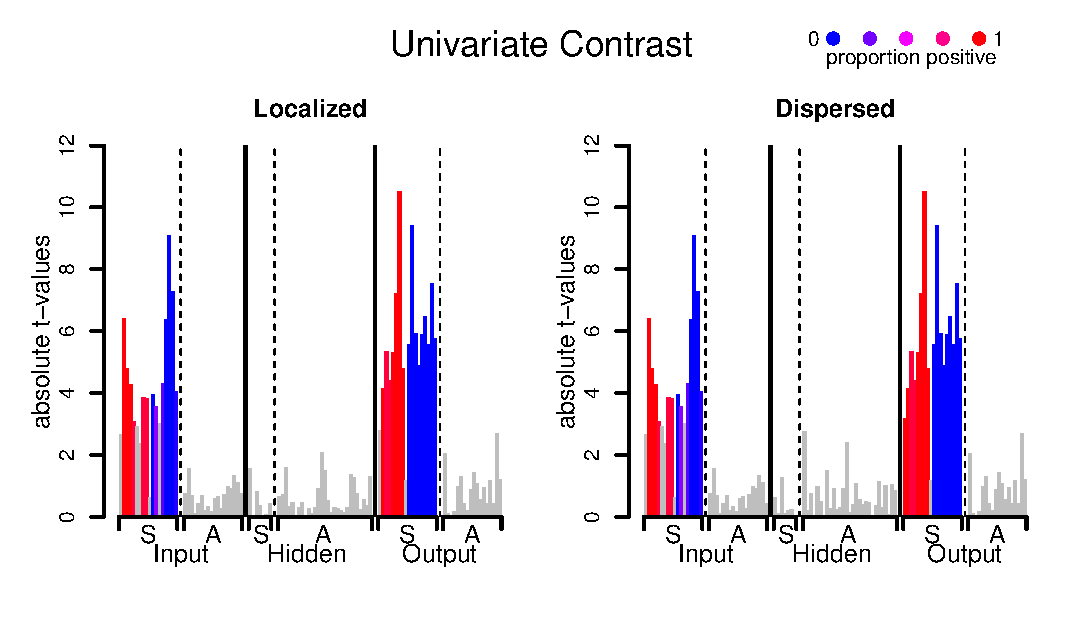
\includegraphics[width=1\textwidth]{figures/univariate.eps}
\caption{\label{fig.univariate} Results from the univariate analysis of simulated data. Bar height indicates the t-value of the voxel-wise contrast between conditions at the group level. Bars in red are significant, p-values corrected to control the false discovery rate at $q<0.05$. In all plots, the distributed condition is created by permuting the units within the hidden layer. For plotting, results are un-permuted back to their original order.}
\end{figure}

Figure \ref{fig.univariate} shows the results of applying the univariate method to the localized (left) and dispersed (right) models. In these plots, each bar corresponds to a single unit in the model (analogous to a single voxel). The bars are ordered according to their functional role in the network, as indicated by the X-axis labels. Colored bars indicate units showing statistically significant differences in mean activation across model individuals, while grey bars indicate units that did not show significant differences. Among the colored bars, red indicates units where activation was reliably higher for domain A, and B indicates units where activation was reliably higher for domain B. Note that, in the ``dispersed'' plot (right), the units are shown in their standard functional location for ease of interpretation.

In both localized and dispersed cases, the univariate contrast method identifies systematic I/O units as important for representing the A/B distinction, and correctly indicates that different subsets of input units code this information differently (some responding more to A than B and others showing the opposite pattern). Note that these are the units for which the five univariate assumptions about representation are all valid. In both localized and dispersed cases, however, the analysis completely misses the systematic hidden units, even though these jointly encode a cleaner representation of the A/B domain structure. The failure arises because, in both cases, the univariate assumptions are invalid. When hidden units are localized, assumptions 2 and 4 are violated: the way individual units encode information can vary across SH units in the same model individual, and across individuals at the same anatomical location. When the units are anatomically dispersed, assumption 3 is also invalid: the representation is coded in different anatomical locations across individuals. Because of these departures from the statistical assumptions, the mean activation of a unit at a given anatomical location across individuals does not differ reliably for SH units, even though these do reliably encode the domain distinction in each individual.

In summary, we get the following answers to the core questions:

\begin{enumerate}
\item {\bf Does the method reliably identify the systematic I/O units?} Yes.
\item {\bf Does the method reliably identify the systematic hidden units?} No.
\item {\bf Does the method indicate how the information of interest is coded across identified units?} Yes.
\item {\bf Do method results depend on anatomical localization of signal-carrying units?} No---hidden units are not discovered regardless of anatomical layout.
\end{enumerate}
